\documentclass[a4paper,10pt]{article}
\usepackage{graphicx,wrapfig,hyperref}
\usepackage[hmargin=3.5cm,vmargin=3.0cm]{geometry}
\begin{document}

\title{TI2800 Contextproject - My Cultural Heritage\\ Requirements Analysis and Design}
\author{Sjoerd van Bekhoven\\ Tim Eversdijk \\ Herman Blanken \\ Rutger Plak \and 4014774 \\ 4005562 \\ 4078624 \\ 1358375}

\maketitle
\setcounter{page}{0}
\thispagestyle{empty}
\vspace{10cm}
		\begin{figure}[ht!]
				\centering
				
\includegraphics[width=\textwidth]{cultuurapp-logo.png}
			\end{figure}
\clearpage

\tableofcontents

\clearpage
\section{Introductie}
Het systeem zal toeristen op een aantrekkelijke manier van zo nuttig mogelijke informatie gaan voorzien van verschillende monumenten. Deze doelen zullen op verschillende manieren worden bereikt. Deze manieren staan beschreven in hoofdstuk 2.

\clearpage
	\section{Overzicht}
		\subsection{Front-end}
			De front-end van de applicatie focus zich op twee punten:
			\begin{enumerate}
				\item Het aantrekkelijk weergeven van de informatie die we vergaard hebben van de monumenten.
				\item Het systeem zo intu\"itief mogelijk laten werken en weergeven.
			\end{enumerate}
				
		\subsection{Back-end}
			De back-end focust zich op het vergaren van nieuwe informatie voor ons systeem. Dit gebeurt op meerdere manieren:
			\begin{itemize}
				\item Niet alle monumenten hebben standaard een categorie aan zich gelinkt. De back-end zal door middel van beeld- en tekstanalyse bepalen in welke categorie het monument ingedeeld moet worden.
				\item Foto's van de monumenten zullen van Flickr en Wikimedia Commons gehaald worden.
				\item Data en foto's worden via de API van rijksmonumenten.nl opgehaald.
				\item Er wordt user-interactie-informatie bijgehouden.
				\item User-interactie-informatie wordt verwerkt tot bruikbare informatie, zoals bijvoorbeeld voorkeuren van users of applicatie brede aanbevelingen en sorteringen.
			\end{itemize}
			
		\clearpage
		\section{Functional requirements}
            \subsection{Zoeken van relevante Flickr-foto's}
            \begin{enumerate}
                \item Er is een systeemcomponent dat live foto's kan ophalen van Flickr\footnote{http://www.flickr.com/services/api/} aan de hand van de geografische locatie, tags en zoektermen.
                \item De website toont foto's uit de buurt van het monument van Flickr wanneer een toerist de detailpagina van een monument bezoekt. Deze foto's worden opgehaald bij het bezoeken van de detailpagina en alleen de url van de foto's worden opgeslagen.
            \end{enumerate}
            
            \subsection{Completeren dataset}
            \begin{enumerate}
                \item Foto's kunnen offline worden geanalyseerd door middel van visuele analyse. Hiervoor wordt ImageJ\footnote{http://rsbweb.nih.gov/ij/} gebruikt. De resultaten van de analyse worden naar de server ge-upload.
                \item Tekst kan online worden geanalyseerd met Naive Bayesiaanse filters. Indien er een dienst wordt gevonden die dit kan doen (uClassify.com is een kandidaat) dan wordt deze gebruikt, zo niet dan wordt dit ge\"implementeerd.
                \item Aan de hand van de resultaten van de visuele en textuele analyse worden monumenten gekoppeld aan bestaande categorie\"en, namelijk die van andere monumenten.
                \item De toerist kan zoeken naar vergelijkbare monumenten. De resultaten van de visuele en textuele analyse tellen mee in de volgorde van de resultaten. Ook de locatie, titel en categorie en gebruikers-interactie-informatie speelt mee.
            \end{enumerate}
    
            \subsection{Foursquare}
            \begin{enumerate}
                \item Het systeem kan controleren of er voor een monument een FourSquare 'venue' (de naam van een locatie op FourSquare) bestaat.
                \item Het systeem kan een FourSquare venue aanmaken indien dit voor een monument nog niet bestaat.
                \item De website toont het aantal check-ins bij de venue.
                \item De website slaat bij het bezoeken van de detailpagina van een monument het meest recente aantal check-ins op FourSquare op.
                \item Een beheerder kan voor een hele set toegevoegde monumenten FourSquare locaties aan laten maken en check-ins laten controleren. Dit kan ook ingepland worden.
            \end{enumerate}
                
            \subsection{Weersinformatie}
            Op de detail pagina zal een weersverwachting staan van de omgeving rond de locatie van het betreffende monument. Deze weersverwachting zal worden opgehaald van Wunderground waar de longitude en latitude van het monument aan mee zal worden gegeven.
            \begin{enumerate}
            \item Er is een systeemcomponent welke live door middel van het meegeven van de longitude en latitude van een locatie de weersverwachting voor deze locatie kan ophalen van Wunderground\footnote{http://dutch.wunderground.com/weather/api/}.
            \item Op de detailpagina wordt de weersverwachting rond het monument getoond.
            \end{enumerate}
                
            \subsection{Faciliteiten rond monument-locatie}
            Op de detail pagina zal de optie zijn faciliteiten in de buurt van het betreffende monument op het kaartje te weergeven. Deze faciliteiten worden opgevraagd bij Google Places\footnote{http://code.google.com/apis/maps/documentation/places/}. Hier zal weer de longitude en de latitude van het monument aan worden meegegeven. De toerist kan aangeven wat voor categorie\"en hij op de kaart wil zien verschijnen. De categorie\"en waaruit gekozen kan worden zijn nader te bepalen.
            \begin{enumerate}
            \item Er is een systeemcomponent welke door middel van het meegeven van een longitude en latitude van een locatie en een faciliteit categorie faciliteiten in de buurt van deze locatie bij Google Places kan ophalen.
            \item Op de detailpagina worden faciliteiten getoond op een kaartje van de omgeving rondom het monument.
	  \item  Op de overzichtspagina worden faciliteiten getoond. De toerist kan aangeven welke categorie\"en faciliteiten getoond moeten worden op het kaartje.
            \end{enumerate}
                
            \subsection{Monumenten vergelijken aan de hand van foto's}
	  \begin{enumerate}
		\item Er is een lokaal systeem dat nog niet geanalyseerde foto's kan ophalen van de webserver en deze kan analyseren met behulp van de Java-tool ImageJ\footnote{http://rsbweb.nih.gov/ij/}.
		\item Het lokale systeem kan de resultaten van de analyse uploaden naar de webserver.
		\item De webserver kan zoeken in de resultaten van de analyse om bij \'e\'en afbeelding andere afbeeldingen te vinden die gelijkend zijn.
		\item Het lokale systeem kan de resultaten van de analyse visueel uitzetten met behulp van de Java-tool  ImagePlot\footnote{http://lab.softwarestudies.com/p/imageplot.html}.
		\item Vanuit het lokale systeem zijn nog niet gecategoriseerde monumenten snel handmatig in te delen in categorie\"en door ze te groeperen aan de hand van de resultaten van de visuele analyse.
		\item De toerist kan onderaan de detailpagina visueel vergelijkbare monumenten bekijken.
	  \end{enumerate}
	                
            \subsection{Implementeren thesaurus}
            De nader te bepalen methode van tekstuele analyse wordt nauwkeuriger door het gebruik van een thesaurus, bijvoorbeeld Cornetto\footnote{http://semanticweb.cs.vu.nl/europeana/browse/list\_graph?graph=http://purl.org/vocabularies/cornetto/cornetto-wn30.ttl.gz}. Tekstueel niet gelijkende woorden kunnen zeer relevant zijn. Zonder thesaurus kunnen deze links niet worden gelegd, met thesaurus kunnen hierdoor teksten op een hoger niveau worden geanalyseerd en kan er nauwkeurigere informatie worden gegeven door het systeem.
\begin{enumerate}
\item Er zal een systeem component zijn welke links kan leggen tussen woorden welke textueel niet gelijkend zijn maar toch erg relevant. Een woord zal worden meegegeven aan dit component en mocht deze bepaalde links hebben opgeslagen met dit woord een lijstje relevante woorden terug geven.
\end{enumerate}

	\subsection{Monumenten filteren}
	\begin{enumerate}
		\item Toeristen kunnen monumenten filteren op aftand tot hun huidige locatie. De toerist geeft een bepaalde afstand aan waardoor alle monumenten die buiten deze aftand tot de huidige locatie weg gefilterd worden. Deze filter methode is alleen toegankelijk wanneer het opvragen van de huidige locatie door het systeem is geslaagd.
		\item Toeristen kunnen monumenten filteren op afstand tot een opgegeven locatie. De toerist geeft een locatie op in de vorm van een adres en geeft vervolgens een bepaalde afstand aan. Alle monumenten buiten deze afstand tot het adres worden weg gefilterd.
		\item Toeristen kunnen monumenten filteren op naam. De toerist zal een tekst opgeven waardoor vervolgens alleen de monumenten overblijven waar deze tekst volledig of deels voorkomt in de monument naam. Deze monumenten zullen gesorteerd worden op textueele relevantie.
		\item Toeristen kunnen monumenten filteren op Populariteit. De toerist geeft een bepaald populariteits niveau op en alle monumenten welke hier buitenvallen worden weg gefilterd. De overgebleven monumenten worden gesorteerd op populariteit mits er niet gefilterd word op naam. 
	\end{enumerate}
        
            \subsection{Kaarten}
			De toerist moet monumenten op een kaart van Google Maps\footnote{http://code.google.com/apis/maps/index.html} kunnen bekijken. De monumenten worden als spelden op de kaart geplaatst. Aan de hand van de door de toerist ingevoerde selectiecriteria wordt een set monumenten geselecteerd. Van deze set wordt aan Google Maps de GPS locaties gegeven. Google Maps retourneert een kaart met de betreffende spelden. De locatie van de toerist wordt opgevraagd, indien deze beschikbaar is wordt deze locatie ook op de kaart getoond.

			\subsection{Overzichtsweergave}
			De toerist moet monumenten in een overzichtsweergave kunnen bekijken. De monumenten worden als rijen getoond informatie getoond. Hierin staat een thumbnail van het monument, de titel en een korte beschrijving. Wanneer de toerist op een rij klikt komt hij op de detailpagina.
			Aan de hand van de door de toerist ingevoerde selectiecriteria wordt een set monumenten geselecteerd.  Beschikbare sorteercriteria voor de lijst monumenten:
			\begin{enumerate}
			\item Afstand tot  locatie
			\begin{itemize}
			\item Afstand tot huidige locatie (indien beschikbaar)
			\item Afstand tot door de toerist gespecificeerde locatie
			\end{itemize}
			\item Naam
			\item Populariteit
			\begin{itemize}
			\item De populariteit van een monument wordt berekend aan de hand van het aantal Foursquare checkins, aantal maal bekeken op de website en het aantal maal gefavoriet. 
			\end{itemize}
			\item Jaartal
			\end{enumerate}
			
            \subsection{Inloggen}
            Toeristen kunnen inloggen met behulp van inlogsystemen van derden. OpenID en Facebook zullen in ieder geval worden ondersteund. Dit verlaagt de drempel voor het maken van een account omdat een toerist geen extra gegevens hoeft te onthouden.
\begin{enumerate}
\item Touristen kunnen op het systeem inloggen via hun Facebook account. Dit gebeurd door de facebook gebruikersnaam en wachtwoord naar de api van facebook te sturen.
\item Touristen kunnen op het systeem inloggen via hun OpenID account. Dit gebeurd door de OpenID gebruikersnaam en wachtwoord naar de api van OpenID te sturen.
\item Touristen kunnen een eigen cultuurapp account aanmaken op het systeem door hun email adres en een wachtwoord in te vullen.
\item Toeristen kunnen op het systeem inloggen met hun cultuurapp account. Dit gebeurd door de cultuurapp account naam en wachtwoord te verifieren door het systeem.
\end{enumerate}
		
		\clearpage
		\section{Nonfunctional requirements}
			Hieronder wordt ingegaan op de non-functional requirements toegankelijkheid, onderhoudbaarheid en betrouwbaarheid.\\	\\
			\textit{Toegankelijkheid}\\
			Er is een centrale server waar alle berekeningen worden uitgevoerd met specifieke software. De client heeft slechts een webkit of Gecko internetbrowser met een javascript engine. Dit betekent dat het op iedere computer / handheld met een gerenomeerde webbrowser (Google Chrome, Mozilla Firefox, Safari) werkt. Op een handheld device, zoals een iPhone of Android toestel, zal het systeem ook werken. Op deze manier is de applicatie voor zoveel mogelijk mensen bruikbaar. Een toerist kan het systeem thuis gebruiken, maar ook op locatie (mits verbonden met internet).\\ \\
			\textit{Onderhoudbaarheid}\\
			De onderhoudbaarheid geeft aan in hoeverre het eenvoudig, moeilijk, goedkoop of duur is om het systeem in een later stadium aan te passen om aan nieuwe requirements te voldoen of fouten te herstellen. De ontwikkelomgeving die we gebruiken maakt het mogelijk om eenvoudig aanpassingen te maken aan het systeem. De inspanningen bij onderhoud zullen dan ook gering zijn.\\ \\
			\textit{Betrouwbaarheid}\\
			De data die gebruikt wordt ligt grotendeels vast in de database. De database wordt dynamisch bijgewerkt wanneer een toerist interfereert met het systeem. De database zal eenmaaldaags gebackupt worden naar een andere server. Bij een eventuele crash van het systeem waarbij schade aan de database zou optreden zullen alleen wijzigingen van maximaal 24 uur verdwijnen. Deze wijzigingen zijn echter geen triviale informatie voor het systeem, zij zullen het systeem alleen helpen bij het accurater tonen van informatie. Wanneer een externe databron niet beschikbaar is, zal slechts een module of feature van de website (zoals nabije hotels tonen) niet werken. Slechts wanneer Google Maps niet meer werkt, zal een grote visuele feature van de software niet beschikbaar zijn. Met een up-time van minimaal 99,9\%\footnote{http://www.google.com/enterprise/earthmaps/maps-sla.html} komt dat neer op maximaal 90 seconden per dag, in de praktijk merkt een toerist hier niets van.
			
		\clearpage
		\section{Constraints ("Pseudo requirements")}
			De pseudo-requirements delen we onder in de serverside en de clientside:
			\begin{itemize}
				\item De back-end van de software zal draaien op een Debian Linux machine met een Apache webserver. Visuele gelijkenissen en verschillen worden onderzocht met de objectgeori\"enteerde programmeertaal Java. De data zal worden opgeslagen in een (My)SQL database. Voor het afhandelen van verzoeken van de client wordt de programmeertaal PHP gebruikt.
				\item Aan de kant van de client wordt data opgehaald in HTML formaat. Hierin wordt de website opgebouwd met behulp van CSS. Om dynamisch dingen op de site te tonen of veranderen wordt JavaScript gebruikt.
			\end{itemize}
		
		\clearpage
		\section{Analysis models}
		\subsection{Use case models, descriptions and scenarios}
			\subsubsection{Use case: selecteren}
			\textit{Doel}\\
			Het doel is de toerist op een eenvoudige wijze monumenten te laten zoeken aan de hand van verschillende criteria. De toerist moet aan de hand van zijn interesses de hoeveelheid monumenten verlagen zodat eenvoudig de interesses naar voren komen in de getoonde monumenten.\\ \\
			\textit{Samenvatting}\\
			"Als toerist wil ik aan de hand van verschillende selectiecriteria de monumenten in de resultaatpagina beperken:
			\begin{itemize}
				\item Wanneer ik kaartweergave gebruik, moeten spelden verdwijnen of verschijnen afhankelijk van of de monumenten die deze spelden verantwoorden aan deze selectiecriteria voldoen.
				\item Wanneer ik overzichtsweergave gebruik, moeten rijen informatie verdwijnen of verschijnen afhankelijk vam of de monumenten die deze rijen informatie verantwoorden aan deze selectiecriteria voldoen."
			\end{itemize}
			\textit{Actoren}\\
			Toerist\\ \\
			\textit{Precondities}\\
			De set met getoonde monumenten is de set van alle monumenten.\\
			\{ type monument, locatie, naam, populariteit, trefwoorden, jaartal \} \\ \\
			\textit{Triggers}\\
			Deze use case wordt getriggerd zodra de toerist een of meerdere selectiecriteria invult.\\ \\
			\textit{Post condities}\\			
			De input van de toerist wordt omgezet naar een set monumenten die aan de selectie voldoen. In de kaartweergave zal dit betekenen dat de hoeveelheid spelden verminderd. In de overzichtsweergave zal dit betekenen dat de hoeveelheid informatierijen verminderd.		
			
			\subsubsection{Use case: informatie}
			\textit{Doel}\\
			Het doel is de toerist op een overzichtelijke en natuurlijke manier van informatie over het geselecteerde monument te voorzien. De toerist moet nuttige informatie te zien krijgen. Ook moet hij informatie te zien krijgen die hem kunnen helpen bij het bezoeken van het monument.\\ \\
			\textit{Samenvatting}\\
			"Als toerist wil ik wanneer ik op een speld op de kaart, of informatierij in de overzichtsweergave klik, verwezen worden naar de pagina met informatie over het monument die de speld of informatierij verantwoord. Op deze pagina wil ik de informatie beschreven in figuur \ref{interface3} op pagina \pageref{interface3} te zien krijgen. Ik wil een kaartje te zien krijgen waarin is ingezoomd op het monument. Op de kaart wil ik in een straal van x kilometer hotels kunnen zoeken, evenals restaurants, barretjes en andere monumenten. Ik wil dat het systeem mijn interesses bepaald en aan de hand van mijn interesses monumenten aanraadt waar ik in ge\"interesseerd ben."\\ \\
			\textit{Actoren}\\
			Toerist\\ \\
			\textit{Precondities}\\
			De toerist weet niets van het geselecteerde monument.\\ \\
			\textit{Triggers}\\
			Deze use case beschrijft de situatie waarin de toerist een monument selecteert. In de overzichtsweergave gebeurt dit wanneer een informatierij die een monument vertegenwoordigt aangeklikt wordt. In de kaartweergave gebeurt dit bij het aanklikken van een speld die een monument vertegenwoordigt.\\ \\
			\textit{Post condities}\\
			De toerist weet veel over het monument en heeft alle informatie die de toerist nodig heeft wanneer de toerist het monument zou willen bezoeken.	
			
			\subsubsection{Use case: mobiliteit}
			\textit{Doel}\\
			De toerist op locatie voorzien van informatie en het mogelijk maken foto's toe te voegen aan het systeem.\\ \\
			\textit{Samenvatting}\\
			"Als toerist wil ik wanneer ik op de plaats van bestemming ben aangekomen met behulp van mijn mobiele apparaat een foto kunnen uploaden / twitteren die door het systeem wordt toegevoegd aan de foto's die bij het monument horen. Ik wil hierbij steekwoorden kunnen meegeven die door het systeem worden herkend. Wanneer ik via dit mobiele systeem een monument, hotel, bar, of ander point of interest selecteer, wil ik dat het navigatieprogramma van mijn mobiele apparaat automatisch opent, zodat ik hier eenvoudig naar toe geleid wordt."\\ \\
			\textit{Actoren}\\
			Toerist\\ \\
			\textit{Precondities}\\
			De toerist is onderweg en wil informatie opzoeken. De toerist heeft op zijn mobiele apparaat een internetverbinding waarmee de toerist het systeem kan raadplegen.\\ \\
			\textit{Triggers}\\
			De toerist gebruikt zijn mobiele apparaat om een monument te selecteren. Dit kan aan de hand van de selectieprocedure beschreven in use case 1, maar ook aan de hand van een lijst favoriete monumenten die aangemaakt kan worden zoals beschreven in use case 4.\\ \\
			\textit{Post condities}\\
			De toerist heeft op locatie toegang tot informatie. Het systeem heeft extra foto's.	
			
			\subsubsection{Use case: favorieten}
			\textit{Doel}\\
			De toerist zijn favoriete monumenten eenvoudig terug te laten vinden.\\ \\
			\textit{Samenvatting}\\
			"Als toerist wil ik wanneer ik een monument heb gevonden dat ik graag zou willen bezoeken of op een later tijdstip nogmaals wil bekijken, dat ik dit monument aan een lijst kan toevoegen. Deze lijst wil ik altijd kunnen raadplegen na inloggen met mijn gebruikersnaam en wachtwoord of OpenID. Wanneer ik onderweg ben, wil ik op mijn mobiele apparaat kunnen inloggen en alle beschikbare informatie over dit monument kunnen zien. Wel wil ik zelf kunnen bepalen of andere toeristen mijn lijst met monumenten kunnen bekijken."\\ \\
			\textit{Actoren}\\
			Toerist\\ \\
			\textit{Precondities}\\
			De toerist heeft monumenten gevonden.\\ \\
			\textit{Triggers}\\
			De toerist voegt een monument toe aan zijn favorieten.\\ \\
			\textit{Post condities}\\
			De toerist kan inloggen om zijn lijst favoriete monumenten te raadplegen.	
			
			\subsubsection{Use case: toevoegen foto's}
			\textit{Doel}\\
			De toerist extra foto's laten toevoegen aan de database.\\ \\
			\textit{Samenvatting}\\
			"Als toerist wil ik als ik bij een monument ben een foto kunnen maken en deze op kunnen slaan in de database. Dit wil ik doen door vanuit de mobiele applicatie een foto te maken en te uploaden. Ook kan een toerist zodra hij of zij thuis komt foto's van een monument uploaden."\\ \\
			\textit{Actoren}\\
			Toerist\\ \\
			\textit{Precondities}\\
			De toerist is bij het monument en maakt een foto\\ \\
			\textit{Triggers}\\
			De toerist upload een foto.\\ \\
			\textit{Post condities}\\
			De foto is toegevoegd aan de database van foto's die bij het monument horen.
	\subsection{Business object model}
		Zie figuur \ref{bom}.
		\begin{figure}[ht!]
			\centering
			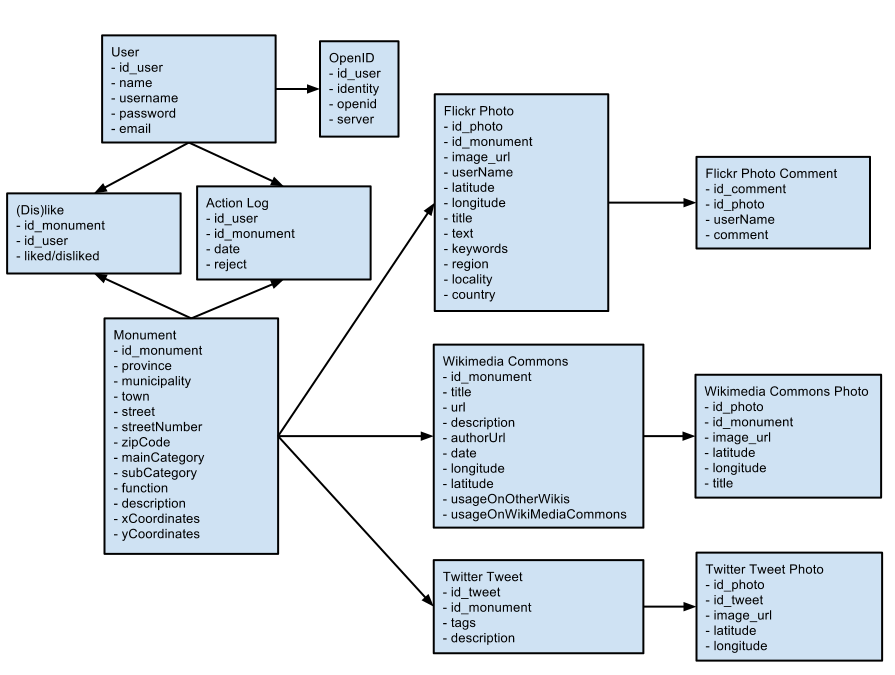
\includegraphics[width=\textwidth]{BusinessObjectModel.png}
			\caption{Business Object Model \label{bom}}
		\end{figure}
		\subsection{Dynamische modellen}
			Belangrijke scenario's beschreven met sequence, state of activity diagrammen.
			\subsubsection{Sequence diagram 1}
			De toerist start de applicatie en komt uit op de pagina waarop de toerist monumenten ziet en selectiecriteria kan gebruiken, zie figuur .. %\ref{sequence1}.
			\begin{figure}[ht!]
				\centering
				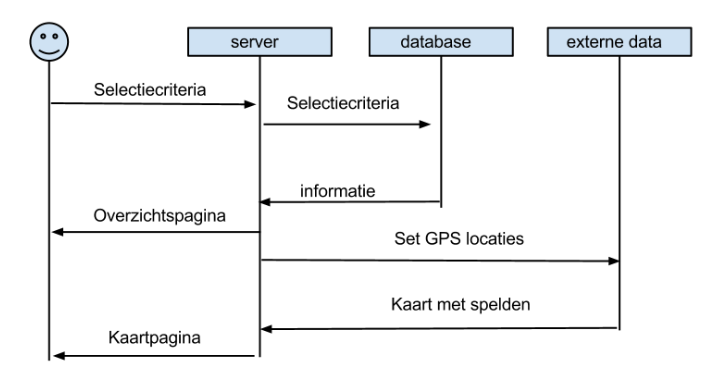
\includegraphics[width=\textwidth]{sequence1.png}
				\caption{Sequence Diagram 1 \label{sequence1}}
			\end{figure}
			\subsubsection{Sequence diagram 2}
			De toerist heeft een monument geselecteerd en komt uit op de detailpagina, zie figuur \ref{sequence2}.
			\begin{figure}[ht!]
				\centering
				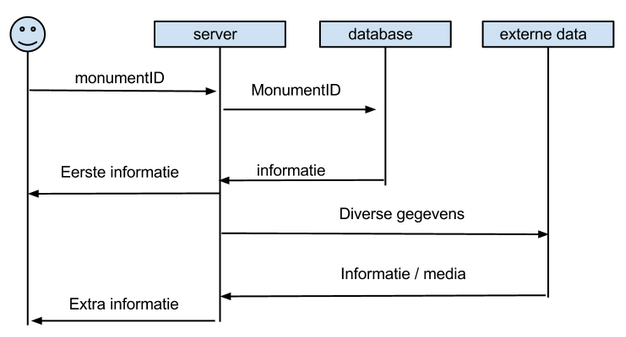
\includegraphics[width=\textwidth]{sequence2.png}
				\caption{Sequence Diagram 2 \label{sequence2}}
			\end{figure}
			\subsubsection{Sequence diagram 3}
			De toerist tweet een foto van een monument aan de hand van \#cultuurapp \#monumentID, zie figuur \ref{sequence3}.
			\begin{figure}[ht!]
				\centering
				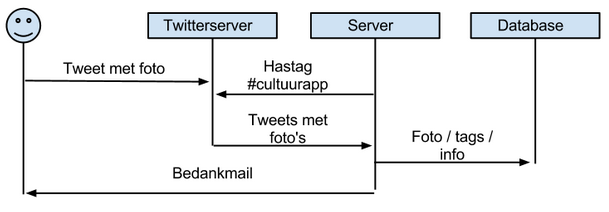
\includegraphics[width=\textwidth]{sequence3.png}
				\caption{Sequence Diagram 3 \label{sequence3}}
			\end{figure}
		
		\clearpage			
		\section{User interface}
			\subsection{Interface 1}
			De toerist start de applicatie en komt uit op een pagina met monumenten die de toerist kan filteren aan de hand van selectiecriteria. De toerist kan schakelen tussen twee view-mogelijkheden, namelijk de kaart met monumenten (figuur \ref{interface1}) of de overzichtspagina met monumenten (figuur \ref{interface2}). De toerist kan hierbij selecteren op een aantal criteria:\\
			\\
			\textit{Monument-type}\\
			Wanneer de toerist het type monument wil selecteren, kan hij in een lijst van monumenttypes een of meerdere types aanvinken.\\
			\\
			\textit{Locatie}
			\begin{itemize}
				\item Op GPS of WIFI gebaseerde huidige locatie: de huidige locatie van de toerist kan worden berekend door het systeem. Wanneer deze optie wordt gebruikt, wordt automatisch de straal ingevuld met een standaardwaarde. 
				\item Provincie / plaats / straat: De toerist kan in een veld een adres, straat of provincie invoeren. Wanneer deze optie wordt gebruikt, wordt automatisch de straal ingevuld met een standaardwaarde.
				\item Straal om de locatie: in combinatie met een gekozen locatie (ingevoerd of berekend) kan een gebied worden aangegeven waarin het systeem monumenten moet weergeven. Alleen de monumenten binnen het ingevuld aantal kilometers van de gekozen of berekende locatie worden getoond door het systeem.
				\item Te bereiken binnen x tijd met ov: Deze optie is alleen beschikbaar als er een locatie is berekend of ingevoerd. De toerist kan een tijdsspan invullen. Het systeem toont slechts de monumenten die binnen de ingevoerde tijdsspan met het openbaar vervoer bereikt kunnen worden.
				\item Te bereiken binnen x tijd met de auto: Deze optie is alleen beschikbaar als er een locatie is berekend of ingevoerd. De toerist kan een tijdsspan invullen. Het systeem toont slechts de monumenten die binnen de ingevoerde tijdsspan met de auto bereikt kunnen worden.
			\end{itemize}
			\textit{Naam}\\
			De toerist kan een (gedeeltelijke) naam invoeren van een monument. Alleen de monumenten met (gedeeltelijk) deze ingevoerde naam worden door het systeem getoond. Bij invoer van 'abc' worden zowel monumenten 'abc', 'abcdef' als 'qweabc' getoond.\\
			\\
			\textit{Populariteit}\\
			De populariteit van een monument wordt door het systeem berekend aan de hand van hoe vaak een monument bezocht wordt, in verhouding met hoeveel monumenten er in een straal van x kilometer ligt. Met een schuifbalk kan de toerist meer / minder monumenten tonen door een minimum populariteit op te geven.\\
			\\
			\textit{Trefwoorden}\\
			De toerist kan trefwoorden invoeren waarop de toerist wil zoeken. Alleen de monumenten die (in een van de bronnen) de ingevoerde woorden bevatten worden getoond.\\
			\\
			\textit{Indoor/outdoor}\\
			De toerist kan ingeven of hij een indoor of een outdoor monument zoekt. Bij keuze van indoor worden alleen monumenten getoond die indoor zijn. Bij keuze van outdoor worden alleen monumenten getoond die outdoor zijn. Bijvoorbeeld bruggen wegen of ruines zijn leuk om te zoeken bij mooi weer. Kerken en musea zijn ook leuk om te bezoeken bij slecht weer. De categorisatie wordt gedaan aan de hand van zowel tekstuele als visuele informatie van het document.\\
			\\
			\textit{Jaartal}\\
			De toerist kan een periode opgeven waarin het bouwjaar van een monument moet liggen. Alleen de monumenten die tussen de randwaarden zijn gebouwd worden getoond op de kaart.
			\subsection{Interface 2}
			Wanneer de toerist een monument heeft geselecteerd komt de toerist uit op een detailpagina (figuur \ref{interface3}).\\
			\\
			\textit{Details die altijd bij een monument worden weergeven:}
			\begin{enumerate}
				\item Naam, de naam van het monument.
				\item Omschrijving, een korte omschrijving van het monument.
				\item Plaatje, een plaatje van het monument uit het monumenten register.
				\item Locatie (longitude, latitude), deze zal worden weergeven door middel van een kaartje (google maps).
				\item Provincie, provincie waar het monument zich bevindt.
				\item Gemeente, gemeente waar het monument zich bevindt.
				\item Stad, stad waar het monument zich bevindt.
				\item Postcode, de postcode van het gebied waar het monument zich bevindt.
				\item Datum, de datum van toevoeging in het monumenten register.
				\item Categorie, de categorie van het monument.
			\end{enumerate}
			
			\begin{figure}[ht!]
				\centering
				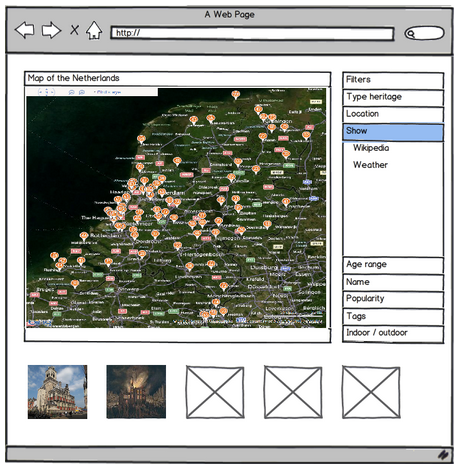
\includegraphics[height=10cm]{interface1.png}
				\caption{Kaart met monumenten \label{interface1}}
			\end{figure}
			
			\begin{figure}[ht!]
				\centering
				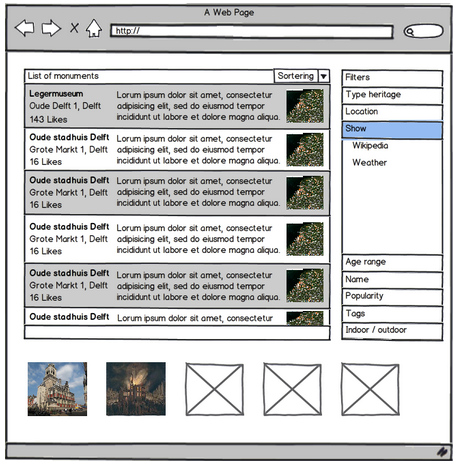
\includegraphics[height=10cm]{interface2.png}
				\caption{Overzichtspagina met monumenten \label{interface2}}
			\end{figure}
			
			\begin{figure}[ht!]
				\centering
				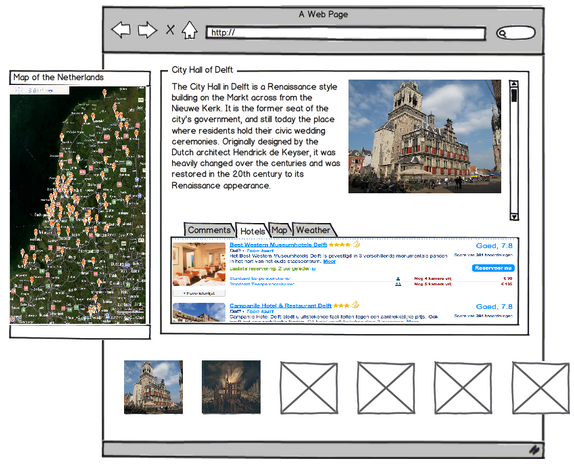
\includegraphics[height=10cm]{interface3.png}
				\caption{Detailpagina monument \label{interface3}}
			\end{figure}
			\textit{Details waarvan het systeem informatie toont wanneer deze berekend kunnen worden / beschikbaar zijn:}
			\begin{enumerate}
				\item Foto's van het monument, op diverse manieren vergaard van diverse data-bronnen.
				\item Weersverwachting voor de locatie van het monument.
				\item Informatie over of het monument overdekt is, of in de open lucht.
			\end{enumerate}
	
	\clearpage
	\section{Glossary}
		\begin{tabular}{ l | l }
		API & Een systeem dat functies en data van het systeem beschikbaar  \\
			& stelt voor de buitenwereld via gedocumenteerde functies.\\
		back-end & de kant van het systeem die de toerist nooit ziet.\\
		check-in& actie op het FourSquare-platform, het aangeven dat een gebruiker  \\
			& zich op een bepaalde locatie op een bepaalde tijd bevindt.\\
		dataset & de set van $\sim$25.000 monumenten die is vrijgegeven voor dit project.\\
		Flickr & website waar personen foto's kunnen delen met anderen.\\
		FourSquare& website en platform waar personen vrienden kunnen laten weten \\
			& waar ze zich bevinden, met spelelement.\\
		front-end & de kant van het systeem die de toerist ziet.\\
		geo-tag & aan een foto gekoppelde locatiegegevens.\\
		user-interactie-informatie& informatie vergaard aan de hand van acties van een gebruiker.\\
		venue & locatie op Foursquare\\
		Wikimedia Commons& website waar miljoenen multimedia bestanden staan verzameld, \\
			& deze zijn door iedereen vrij te gebruiken.\\
		\end{tabular}
\end{document}